\chapter{Industrialisation du produit}
\label{Industrialisation du produit}
\thispagestyle{fancy}
Une fois le processus fonctionnel de notre système défini, on l'industrialise. Cela signifie que l'on crée un ensemble d'outils permettant de l'utiliser de la manière la plus simple possible et en répondant au mieux à la problématique initiale. \\
On soumet deux types d'outils: l'API, qui permet d'utiliser le système d'automatisation de l'investigation, et les outils graphiques, qui accompagnent l'usage de l'API et permettent à l'utilisateur d'interagir avec le programme.  

\section{API}
\label{Industrialisation du produit: API}
L'API que l'on propose est composée de 3 modules principaux:
\begin{description}
	\item [data base] Permet de gérer le stockage et la lecture des données nécessaires à l'exécution des algorithmes d'apprentissage. Deux types de fichiers sont sauvegardés dans la base de donnée: les fichiers logs, qui fournissent l'ensemble des exemples permettant d'entraîner l'algorithme et les fichiers générés par l'algorithme lors de son apprentissage.
	\item [data set] Gère le pré-traitement et le traitement des exemples afin de les structurer pour réaliser l'apprentissage par la suite.
	\item [machine learning] Permet de créer un algorithme d'apprentissage, de l'entraîner et de l'utiliser pour investiguer sur la root cause pour laquelle il a été créé.
\end{description}

La librairie utilise le langage de programmation Python \cite{Python}. \\

\subsection{Pré-traitement et traitement des données}
\label{Industrialisation du produit: API: Pré-traitement et traitement des données}
Le module "Data set" contenu dans l'API permet de pré-traiter les exemples et de les structurer afin de pouvoir réaliser l'apprentissage. 
Le pré-traitement est composé de 5 étapes.
\begin{description}
	\item [Lecture] La première étape du pré-traitement consiste à lire les données contenues dans le fichier log. 
	\item [Échantillonnage] Les fichiers logs générés par MEIGUI lors du déroulement du Filtering Test n'ont pas forcement tous la même période d'échantillonnage. Cela signifie que les exemples que l'on souhaite utiliser pour l'entraînement ne font pas tous la même taille. Or, les spécificités des fonctions de la librairie Scikit-learn utilisées pour l'entraînement nécessite que celles-ci aient le même nombre d'échantillons. Pour cette raison, échantillonne les données extraites des fichiers logs avec le même nombre d'échantillons. Si le nombre d'échantillons contenu dans le fichier log est inférieur au nombre d'échantillons fixé pour l'échantillonnage, on effectue un sur-échantillonnage lorsque celui-ci n'altère les données. 
	\item [Selection des motifs] Au regard de l'architecture fonctionnelle que l'on a définie en partie \ref{Automatisation du processus d'investigation: Achitecture High Level du système proposé}, on doit extraire les motifs caractéristiques d'une root cause dans chaque exemple utilisé. Pour cela, une sélection manuelle du motif est réalisée en amont via une interface graphique (c.f. \ref{Industrialisation du produit: Présentation des outils: Outils graphiques}). A partir des informations retournées par l'IHM, on est en mesure de sélectionner les données correspondant aux motifs, dans chacun de nos exemples. On rappelle que l'on enregistre également des morceaux de la courbe ne correspondant pas au motif d'une root cause, afin d'avoir les deux types de label lors de l'entrainement de l'algorithme.
	\item [Déroulement des données] On déroule ensuite les données afin de pouvoir réaliser de la reconnaissance de motifs sur plusieurs features (c.f. partie ) \ref{Automatisation du processus d'investigation: Étendre le problème à plusieurs dimensions}), i.e. que l'on place chacune des colonnes de notre matrice d'exemples l'une en dessous de l'autre pour obtenir en sortie un vecteur. 
	\item [Tri des données] Enfin, afin de pouvoir mesurer les performances de notre algorithme (c.f. partie \ref{Automatisation du processus d'investigation: Performances de la solution}), on sépare notre base de données d'exemples en deux groupes: le training set et le test set. Le premier sera utilisé pour entraîner notre algorithme, le deuxième pour le tester. 
\end{description}

\subsection{Sélection des motifs lors du pré-traitement des données }
\label{Industrialisation du produit: API: Sélection des motifs pour entrainement}
Comme étudié en partie \ref{Automatisation du processus d'investigation: Reconnaissance de motifs}, la reconnaissance de motifs passe par la sélection des motifs caractéristiques de la root cause que l'on souhaite détecter pour chaque exemple de notre base de donnée. Elle s'accompagne également de  la sélection de sections de la courbe ne présentant pas ce motif afin de pouvoir réaliser l'apprentissage de l'algorithme correctement( c.f. partie \ref{Automatisation du processus d'investigation: Difficultés notoires rencontrées}). Chaque motif sélectionné doit avoir la même taille i.e. le même nombre d'échantillons pour pouvoir réaliser l'entrainement. Cette taille dépend de la largeur globale du motif caractéristique de la root cause étudiée et est déterminée lors de l'utilisation de l'interface graphique présentée partie ... .   

\subsection{Format des données en sortie du pré-traitement des données}
\label{Industrialisation du produit: API: Format des données en sortie du pré-traitement}
On présente dans le tableau \ref {tab: Structure de la base de données d'exemples après prétraitement} la structure des données en sortie du pré traitement des données. On a deux vecteur : un contenant les exemples de motifs et un deuxième contenant le label associé à chaque motif. Le label 1 signifie que le motif lié correspond à un motif caractéristique de la root cause que l'on cherche à détecter; 0 signifie que le motif lié ne correspond pas à un motif caractéristique de la root cause que l'on cherche à détecter. 
\begin{equation}
\begin{blockarray}{cc}
exemples & label \\
\begin{block}{[c][c]}
exemple_1 &  1 \\
exemple_2 & 0 \\
exemple_3 & 0 \\
exemple_4 & 1 \\
... & ... \\
exemple_m & 0 \\
\end{block}
\end{blockarray}
\label {tab: Structure de la base de données d'exemples après prétraitement}
\end{equation}
On retrouve cette structure pour chaque \emph{set} (i.e. \emph{training set} et \emph{test set})
Chaque exemple correspond à une liste qui contient l'ensemble des échantillons contenus dans un motif (c.f. partie \ref{Industrialisation du produit: API: Sélection des motifs pour entrainement}).

\subsection{Module Marchine Learning et librairie scikit-learn}
\label{Industrialisation du produit:  API: Le module Machine Learning}
Le module Machine Learning s'appuie sur l'utilisation de scikit-learn \cite{ScikitLearn}. Il s'agit d'une bibliothèque Open Source développée par l'INRIA (Institut National de Recherche en Informatique et en Automatique \cite{INRIA}). Elle propose de nombreux outils afin de réaliser de la classification (régression logistique, SVM), de la régression (SVR, régression linéaire) et du clustering (i.e. apprentissage non supervisé). Elle est principalement utilisée dans notre cas pour réaliser de classification (i.e. apprentissage supervisé) en utilisant l'algorithme d'apprentissage automatique SVM. Elle est également utilisée afin de construire le \emph{training set} et le \emph{test set}.




\section{Outils graphiques}
\label{Industrialisation du produit: Outils graphiques}
On présente ici les différents outils graphiques permettant de réaliser la construction d'une nouvelle couche root cause (i.e. l'entrainement d'un nouvel algorithme à détecter une root cause particulière), d'investiguer un error name et d'obtenir des informations quant aux performances de l'algorithme. 

\subsection{Pattern selector}
\label{Industrialisation du produit: Outils graphiques: Pattern selection}
Cet outil graphique permet de sélectionner les motifs contenus dans chaque exemple du \emph{training set} durant la phase de pré-traitement des données.  Il permet également  de labelliser les exemples. \\
Il est formé de trois parties:
\begin{itemize}
	\item La première partie (encadré vert de la figure \ref{fig:Interface graphique du pattern selector}) nous donne divers indications sur l'état actuel du pré-traitement des données : la taille du motif actuellement sélectionné, le nom de l'exemple étudié et le nombre d'exemples restant à traiter. 
	\item La seconde partie (encadré rouge de la figure  \ref{fig:Interface graphique du pattern selector}) est la partie graphique de l'interface graphique. Elle affiche les features de l'exemple actuellement étudiée. Dans le cas de la figure  \ref{fig:Interface graphique du pattern selector}, on réalise par exemple l'entraînement de l'algorithme pour que celui-ci puisse reconnaître le motif caractéristique de la root cause "frottement des freins de la hanche". La région en rouge permet de sélectionner le motif qui nous intéresse. D'après la première partie de l'IHM, on a ici sélectionné un motif dont la taille est de 60 échantillons.
	\item La dernière partie (encadré bleu de la figure  \ref{fig:Interface graphique du pattern selector}) est une succession de boutons permettant d'interagir avec les différents exemples. De gauche à droite :   
	\begin{itemize}
		\item Le  bouton "Previous" permet de revenir à l'exemple précédent.
		\item Le bouton "Found" permet d'indiquer au système que le motif est présent sur l'exemple étudié, et qu'il a bien été sélectionné grâce à la région en rouge. Cela revient à labelliser l'exemple (Y = 1, c.f. partie \ref{Industrialisation du produit: API: Format des données en sortie du pré-traitement})
		\item Le bouton "Not Found" permet d'indiquer au système que le motif n'est pas présent sur l'exemple étudié. Cela revient à labelliser l'exemple (Y = 0, c.f. partie \ref{Industrialisation du produit: API: Format des données en sortie du pré-traitement}). Le prochain exemple à étudier s'affiche.
		\item Le bouton en forme d'œil ouvert permet d'activer le mode étendu (c.f. figure \ref{fig:Interface graphique du pattern selector en mode étendu}). Le prochain exemple à étudier s'affiche.
	\end{itemize} 
\end{itemize} 

\begin{figure}[h]
	\centering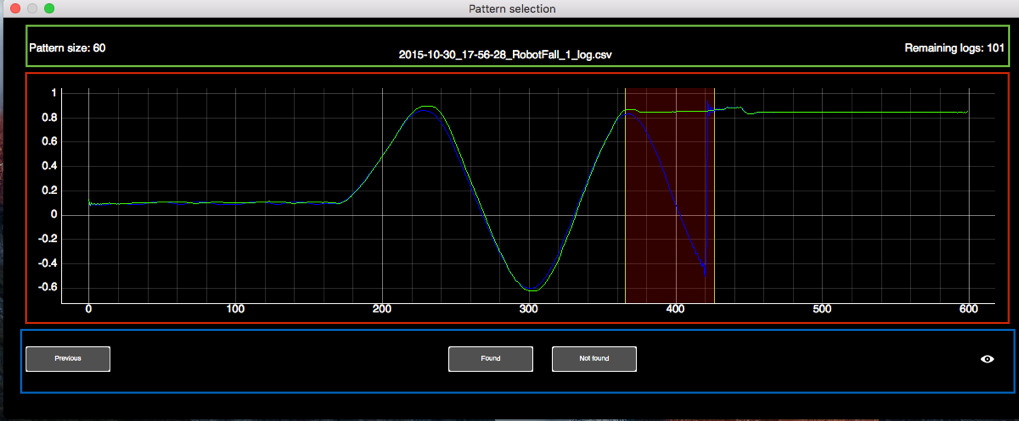
\includegraphics[height=6.4cm]{images/pattern_selector.png}
	\caption[Interface graphique du pattern selector]{Interface graphique du pattern selector.}
	\label{fig:Interface graphique du pattern selector}
\end{figure}

\subsubsection{Région de sélection}
\label{Industrialisation du produit: Outils graphiques: Pattern selection: La région de sélection}
La région de sélection permet de sélectionner le motif caractéristique d'une root cause dans chaque exemple où celui-ci est présent. Il est possible d'augmenter la taille de celui-ci si le besoin est présent. Par exemple, imaginons que l'on sélectionne sur le premier exemple un motif, la taille indiquée en haut à gauche de l'IHM du pattern selector est alors de 60 échantillons. On clique sur le bouton "Found" et un nouvel exemple s'affiche. Celui-ci contient également le motif caractéristique de la root cause que l'on apprend, mais ce dernier est plus large de 10 échantillons. Il est alors possible d'étendre la région de sélection pour pouvoir sélectionner l'ensemble de ce nouveau motif. Cependant, l'ensemble des exemples devant avoir la même taille (même nombre d'échantillons), on modifie la taille des motifs précédemment sélectionnés. Dans le cas de notre exemple, on augmente la taille du motif précédent de 5 échantillons de chaque côté. \\
Il n'est cependant pas possible de réduire la taille d'un motif, afin de ne pas perdre des données sur les exemples précédemment sélectionnés. 

% CREER UNE FIGURE POUR AFFIHCHER PLUS CLAIREMENT

\subsubsection{Mode étendu}
\label{Industrialisation du produit: Outils graphiques: Pattern selection: Mode étendu}
Il existe certains cas où les valeurs de deux features étudiées sont trop éloignées pour pouvoir être visualisé de manière correct. Pour cela, on peut basculer l'IHM en mode étendu, ce qui permet d'afficher chacune des features dans un graphique séparé. La région de sélection est commune aux différents graphe, i.e. sa taille et sa position est contrôlée via le graphique principal et se répercute sur les graphitiques du mode étendu (c.f. figure \ref{fig:Interface graphique du pattern selector en mode étendu})

\begin{figure}[h]
	\centering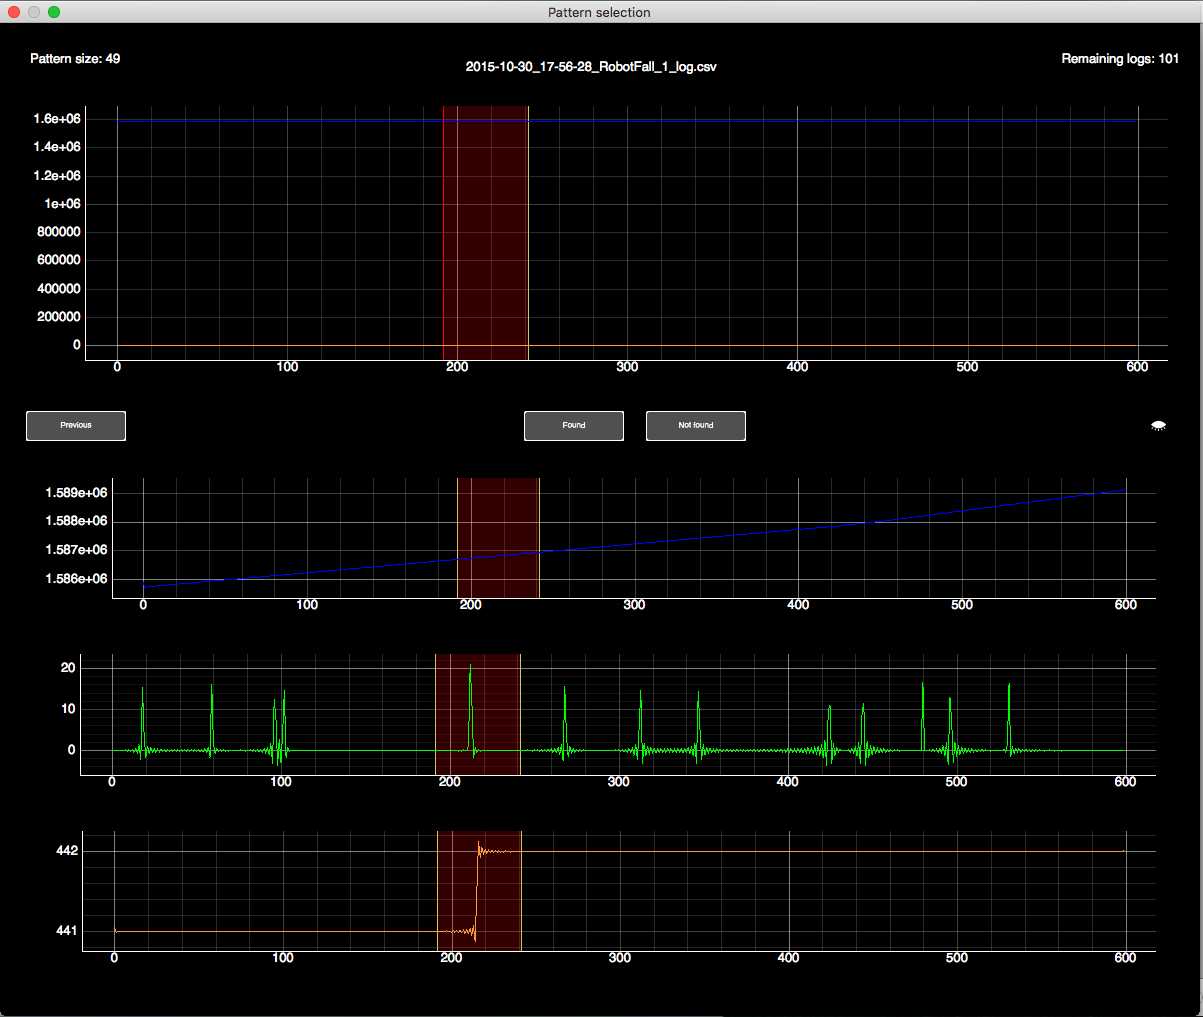
\includegraphics[height=7cm]{images/pattern_selector_ext.png}
	\caption[Interface graphique du pattern selector en mode étendu]{Interface graphique du pattern selector en mode étendu. On observe sur ce graphiques trois features BackPlateformAck, BackPlateformNack et BackPlateformError du premier exemple. On remarque que l'affichage sur le graphique principal n'est pas clair. Le mode étendu permet d'afficher plus clairement chacune des features. La région de sélection est commune aux trois graphiques (même position, même taille).}
	\label{fig:Interface graphique du pattern selector en mode étendu}
\end{figure}

\subsection{Probability Visualization}
\label{Industrialisation du produit: Outils graphiques: Probability Visualization}
Cette interface graphique permet de visualiser l'exemple que l'on investigue et la courbe de probabilité représentant la probabilité que le motif soit présent dans l'image. Celle-ci est composée de deux parties. 
\begin{itemize}
	\item La première partie (encadré vert sur la figure \ref{fig:Interface graphique du probability visualizator}) affiche les features de l'exemple que l'on investigue. Par exemple, dans le cas présenté, on recherche la root cause liée à l'error name "chute du robot". Le système détecte que la root cause liée sur ce cas précis est "le frottement des freins de la hanche". Il nous affiche donc les courbes du senseur et de l'actuateur de la hanche, sur lesquelles on observe le motif caractéristique de la root cause. 
	\item La deuxième partie (encadré rouge sur la figure \ref{fig:Interface graphique du probability visualizator}) affiche la courbe de progression de la probabilité au cours du balayage des features de l'exemple (c.f. partie \ref{Automatisation du processus d'investigation: Reconnaissance de motifs: Concept}). La ligne horizontale sur le graphique représente le seuil à partir du quel on considère que la root cause est bien la cause ayant entraîné l'apparition de l'erreur.
\end{itemize}

\begin{figure}[h]
	\centering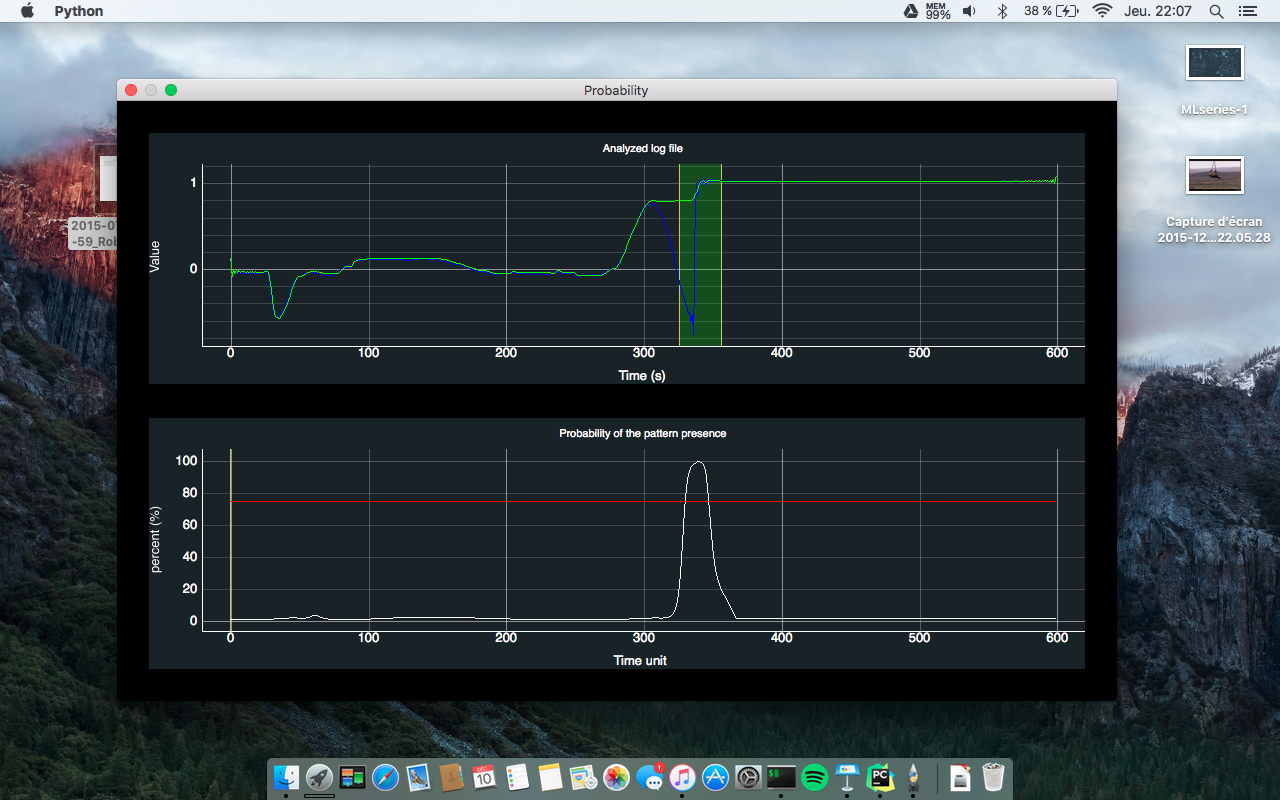
\includegraphics[height=7cm]{images/proba_visu.png}
	\caption[Interface graphique du probability visualizator]{Interface graphique du probability visualizator.}
	\label{fig:Interface graphique du probability visualizator}
\end{figure}

\subsection{Control panel}
\label{Industrialisation du produit: Outils graphiques: Control panel}
Le control panel permet d'obtenir un certain nombre d'informations quant à la qualité de la base de données d'exemple utilisée pour créer une nouvelle couche root cause ainsi que sur les performances de l'algorithme d'apprentissage automatique utilisé. La plupart de ces informations sont déterminées grâce aux outils soumis en partie \ref{Automatisation du processus d'investigation: Performances de la solution}. Il est composé de trois parties.
\begin{itemize}
	\item La partie \emph{Data set features} (encadré vert sur la figure \ref{fig:Interface graphique du control pattern}) fourni un ensemble d'informations sur la base de données d'exemples utilisée pour l'entraînement de l'algorithme d'apprentissage automatique. 
	\item La partie \emph{Training panel features} (encadré rouge sur la figure \ref{fig:Interface graphique du control pattern} nous livre des informations sur  l'algorithme d'apprentissage automatique de la couche root cause analysée (e.g. valeur des paramètres, matrice de confusion, précision, etc). Ces données sont pour la plupart relatives aux explications fournies en partie \ref{Automatisation du processus d'investigation: Performances de la solution}.
	\item La partie \emph{Training panel} (encadré bleu sur la figure \ref{fig:Interface graphique du control pattern}) permet d'analyser les courbes d'apprentissage (c.f. partie \ref{Industrialisation du produit: Performances de la solution:Courbes d'apprentissage}) et les courbes de validation (c.f. partie \ref{Industrialisation du produit: Performances de la solution:Optimisation des paramètres du SVM})
\end{itemize}

\begin{figure}[h]
	\centering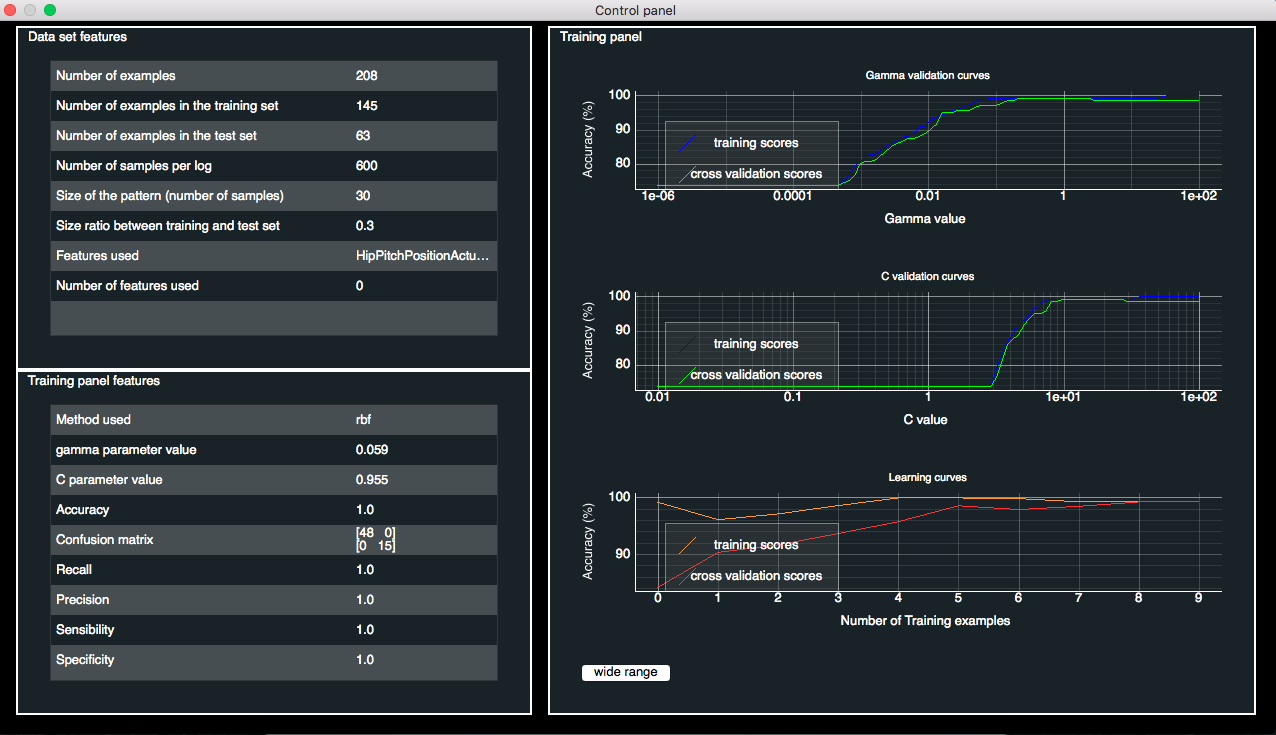
\includegraphics[height=7cm]{images/control_panel.png}
	\caption[Interface graphique du control pattern]{Interface graphique du control pattern.}
	\label{fig:Interface graphique du control pattern}
\end{figure}

\section{Utilisation suggérée des outils pour répondre au problème d'investigation du frottement des freins de la hanche}
\label{Industrialisation du produit: Utilisation suggérée des outils}
On propose dans cette partie un exemple d'utilisation de l'API et des interfaces graphiques. Cette solution a été mise en place dans le cadre du stage afin de proposer un outil permettant dors et déjà de gérer la base de donnée, de créer de nouvelles couches root cause et d'investiguer des fichiers logs. On s'appuie notamment sur l'utilisation de la libraire python \emph{npyscreen} \cite{Npyscreen} qui permet de réaliser des interfaces utilisateurs simplifiées, directement dans le terminal. \\
On s'intéressera ici plus particulièrement au problème de frottement des freins de la hanche, entraînant la chute du robot durant le Filtering Test. Sa résolution passe donc par trois étapes: 
\begin{enumerate}
	\item Créer une nouvelles couche error name : la couche "chute du robot". 
	\item Créer un nouvelle couche root cause liée à la couche error name "chute du robot" : la couche "frottement des freins de la hanche". Cela signifie que l'on va entraîner un nouvel algorithme à détecter le motif caractéristique de cette root cause. 
	\item vérifier les performances de la nouvelle couche root cause créée.
	\item Investiguer un fichier log. 
\end{enumerate}

\subsection{Menu principal}
\label{Industrialisation du produit: Utilisation suggérée des outils: Menu principal}
Le menu principal (c.f. figure )

\subsection{Nouvelle error name}
\label{Industrialisation du produit: Utilisation suggérée des outils: Nouvelle error name}
Le menu "new error name"

\subsection{Nouvelle root cause}
\label{Industrialisation du produit: Utilisation suggérée des outils: Nouvelle root cause}
Le menu "add a root cause to 


\subsection{Performances}
\label{Industrialisation du produit: Utilisation suggérée des outils: Performances}
Le menu principal (c.f. figure )

\subsection{Investiguer}
\label{Industrialisation du produit: Utilisation suggérée des outils: Investiguer}
Le menu principal (c.f. figure )

\subsection{Mise à jour d'une root cause}
\label{Industrialisation du produit: Utilisation suggérée des outils: Mise à jour d'une root cause}
Le menu principal (c.f. figure )



\section{Dimensionnement de la solution}
\label{Industrialisation du produit: Dimensionnement de la solution}